\section{Denotational Model: Groupoid of Groupoids}
\vic{Which is the groupoid of groupoids?}
\label{sec:groupoids}

rig groupoid
objects types
morphisms 1-combinators
coherence conditions 2-combinators

but so far objects are just finite sets essentially
can we get more interesting groupoids such as the ones in the intro
action groupoids

challenge is to find a computational interpretation of action
groupoids: group, group action, ... insight: all we need is to
consider combinators under order; this is a group

also monad/comonad

%%%%%%%%%%%%%%%%%%%%%%%
\subsection{$\Pi$ Semantics: Groupoid of Finite Sets}

From the perspective of category theory, the language $\Pi$ models
what is called a \emph{symmetric bimonoidal category} or a
\emph{commutative rig category}. These are categories with two binary
operations and satisfying the axioms of a commutative rig (i.e., a
commutative ring without negative elements also known as a commutative
semiring) up to coherent isomorphisms. And indeed the types of the
$\Pi$-combinators are precisely the commutative semiring axioms. A
formal way of saying this is that $\Pi$ is the
\emph{categorification}~\cite{math/9802029} of the natural numbers. A
simple (slightly degenerate) example of such categories is the
category of finite sets and permutations in which we interpret every
$\Pi$-type as a finite set, interpret the values as elements in these
finite sets, and interpret the combinators as permutations.

More generally, the types of $\Pi$ are objects that model sets of
natural numbers, the 1-combinators are morphisms that model
cardinality-preserving maps, and the 2-combinators are coherence
conditions on these morphisms~\cite{Carette2016}. The resulting
$\Pi$-category has a rich structure consisting of two symmetric
monoidal structures~\cite{nla.cat-vn1051288} separately induced by the
properties of addition and multiplication of the natural
numbers. These two structures are then augmented with distributivity
and absorption natural isomorphisms~\cite{laplaza} to model the full
commutative semiring (aka, commutative rig) of the natural
numbers. All the morphisms are invertible which makes the resulting
category a ``symmetric rig groupoid''~\cite{nlabrig}.

Despite this rich structure, the individual objects in the category
are just plain sets with no interesting structure. Formally, each
$\Pi$ type $\tau$ induces a finite set $\sem{\tau}$ as follows:

\[\begin{array}{rcl}
\sem{\zt} &=& \bot \\
\sem{\ot} &=& \top \\
\sem{\tau_1 \oplus \tau_2} &=& \sem{\tau_1} \uplus \sem{\tau_2} \\
\sem{\tau_1 \otimes \tau_2} &=& \sem{\tau_1} \times \sem{\tau_2}
\end{array}\]

\noindent where we use $\bot$ to denote the empty set, $\top$ to
denote a set with one element, and $\uplus$ and $\times$ to denote the
disjoint union of sets and the product of sets respectively. Each set
can be viewed as a groupoid whose objects are the set elements and
whose morphisms are just the identity morphisms. By only being able to
express types whose denotations are trivial groupoids, $\Pi$ leaves
untapped an enormous amount of combinatorial structure that should be
within reach. Indeed, as we show next, it is possible with a small but
deep technical insight to extend $\Pi$ with types whose denotations
are non-trivial groupoids such as the ones illustrated in
Fig.~\ref{fig:groupoids}.

%%%%%%%%%%%%%%%%%%%%%%%
\subsection{1-Combinators as Types}

From each 1-combinator $c : \tau \iso \tau$ that maps a type $\tau$ to
itself, we generate two groupoids $\order{p}$ and $\iorder{p}$ with
cardinalities $\mathit{order}(p)$ and $\frac{1}{\mathit{order}(p)}$
respectively. Given that we have sums and products of groupoids, this
small extension allows us to write types whose denotations are
groupoids with the cardinality of an arbitrary positive rational
number. This is in addition to the plain $\Pi$ types whose denotations
are groupoids with the cardinality of an arbitrary natural number. To
make these ideas precise, we first define the cardinality of a
groupoid, and then give the details of the constructions of the
groupoids $\order{p}$ and $\iorder{p}$.

\begin{definition}[Groupoid Cardinality~\cite{2009arXiv0908.4305B}]
  The cardinality of a groupoid $G$ is the real number
  \[
    |G| = \sum_{[x] \in \pi_0(G)} \frac{1}{|\textsf{Aut}(x)|}
  \]
  provided the sum converges, where the sum is over isomorphism classes
  of objects of $G$ and $|\textsf{Aut}(x)|$ is the cardinality or order
  of the automorphism group of an object $x$ in $G$.
\end{definition}

\begin{definition}[Power of a permutation]
  The $k^{th}$ power of a 1-combinator $p : \tau \iso \tau$, for
  $k \in \Z$ is
  \[
    p^k =
  \begin{cases}
    \idiso & k = 0 \\
    p \odot p^{k - 1} & k > 0 \\
    (!~p) \odot p^{k + 1} & k < 0 \\
  \end{cases}
  \]
\end{definition}

\begin{definition}[Order of a permutation]
  The order of a 1-combinator $p : \tau \iso \tau$, $\ord{p}$, is the
  least postitive natural number $k \in \N^+$ such that
  $p^k \isotwo \idiso$.
\end{definition}

\begin{lemma}
  Every $p : \tau \iso \tau$ has an order.
\end{lemma}

\begin{proof}
  By cases.
  \begin{enumerate}
  \item $\ord{\idiso} = 1$
  \item $\ord{\swapp} = \ord{\swapt} = 2$
  \item $\ord{p_1 \odot p_2} = ???$
  \item $\ord{p_1 \oplus p_2} = \ord{p_1 \otimes p_2} = \mathsf{lcm}(\ord{p_1}, \ord{p_2})$
  \end{enumerate}
\end{proof}

\begin{lemma}
  For $p : \tau \iso \tau$, $n \in \Z$, $p^{k + n} \isotwo p^n$ where
  $k = \ord{p}$.
\end{lemma}

\begin{proof}
  Trivial.
\end{proof}

\begin{definition}[$\order{p}$]
  Denotationally, $\order{p}$ is the 1-groupoid whose objects are powers
  of $p$, $p^k$ for $k \in \Z$, and morphisms being 2-combinators
  between them.
\end{definition}

\begin{lemma}
  $|\order{p}| = \ord{p}$
\end{lemma}

\begin{proof}
  Let $k = \ord{p}$. There are $k$ isomorphism classes of
  objects. Consider an object $x = p^n$,
  $\pi_0(x) = p^{n + k}, k \in \Z$. $\textsf{Aut}(x)$ is the group
  generated by $\idisotwo$ and has order 1. Hence
  $|\order{p}| = \sum\limits_{1}^{k}\frac{1}{1} = k$.
\end{proof}

\begin{definition}[$\iorder{p}$]
  Denotationally, $\iorder{p}$ is the 2-groupoid with a zero object
  $\bullet$, morphisms powers of $p$, $p^k$ for $k \in \Z$, and
  2-morphisms being 2-combinators between them.
\end{definition}

\begin{lemma}
  $|\iorder{p}| = 1/\ord{p}$
\end{lemma}

\begin{proof}
  Let $k = \ord{p}$. Consider the object $x =
  \bullet$. $|\texttt{Aut}(x)|$ is the group generated by
  $p^0, p^1 \dots p^{k-1}$, hence $|\iorder{p}| = 1/k$.
\end{proof}

\vic{Should typing judgments be here?}

%%%%%
\subsection{A Universe of Groupoids}

Define action groupoids $\ag{\tau}{p}$ and show they are equivalent to
uparrow tau times 1 over hash p

Talk about monad/comonad ????

each type is a groupoid: discrete and action groupoids
collection of types is another groupoid: commutative semifield

% \begin{code}
% -- Conjecture:  p ⇔ q   implies  order p = order q
% -- Corollary:   p ⇔ !q  implies  order p = order (! q)

% -- The opposite is not true.

% -- Example
% -- p = (1 2 3 4)

% -- compose p 0 = compose !p 0 = compose p 4 = compose !p 4
% -- 1 -> 1
% -- 2 -> 2
% -- 3 -> 3
% -- 4 -> 4

% -- compose p 1  ***     compose !p 1
% -- 1 -> 2       ***     1 -> 4
% -- 2 -> 3       ***     2 -> 1
% -- 3 -> 4       ***     3 -> 2
% -- 4 -> 1       ***     4 -> 3

% -- compose p 2  ***     compose !p 2
% -- 1 -> 3       ***     1 -> 3
% -- 2 -> 4       ***     2 -> 4
% -- 3 -> 1       ***     3 -> 1
% -- 4 -> 2       ***     4 -> 2

% -- compose p 3  ***     compose !p 3
% -- 1 -> 4       ***     1 -> 2
% -- 2 -> 1       ***     2 -> 3
% -- 3 -> 2       ***     3 -> 4
% -- 4 -> 3       ***     4 -> 1

% -- there is a morphism 1 -> 2 using
% -- (compose p 1) and (compose !p 3)
% -- p¹ is the same as !p³
% -- p² is the same as !p²
% -- p³ is the same as !p¹

% data FT/ : Set where
%   ⇑    : FT → FT/
%   #    : {τ : FT} → (p : τ ⟷ τ) → FT/
%   1/#  : {τ : FT} → (p : τ ⟷ τ) → FT/
%   _⊞_  : FT/ → FT/ → FT/
%   _⊠_  : FT/ → FT/ → FT/

% UG : Universe l0 (lsuc l0)
% UG = record {
%     U = FT/
%  ;  El = λ T → Σ[ ℂ ∈ Category l0 l0 l0 ] (Groupoid ℂ)
%  }

% card : FT/ → ℚ
% card (⇑ τ)      = mkRational ∣ τ ∣ 1 {tt}
% card (# p)      = mkRational (order p) 1 {tt}
% card (1/# p)    = mkRational 1 (order p) {order-nz}
% card (T₁ ⊞ T₂)  = (card T₁) ℚ+ (card T₂)
% card (T₁ ⊠ T₂)  = (card T₁) ℚ* (card T₂)
% \end{code}

% %%%%%
% \subsection{Groupoids from $\Pi$-Combinators}

% The goal is to define a function that takes a $T$ in $FT/$ and
% produces something of type $Universe.El~UG~T$, i.e., a particular
% groupoid.

% \begin{code}

% -- First each p is an Agda type
% -- Perm p i is the type that contains the i^th iterate
% -- of p, i.e p^i up to <=>.
% -- the parens in the definition of ^ need to be there!

% _^_ : {τ : FT} → (p : τ ⟷ τ) → (k : ℤ) → (τ ⟷ τ)
% p ^ (+ 0) = id⟷
% p ^ (+ (suc k)) = p ◎ (p ^ (+ k))
% p ^ -[1+ 0 ] = ! p
% p ^ (-[1+ (suc k) ]) = (! p) ◎ (p ^ -[1+ k ])

% -- i.e. Perm is: for all i, any p' such that
% -- p' ⇔ p ^ i

% record Perm {τ : FT} (p : τ ⟷ τ) : Set where
%   constructor perm
%   field
%     iter : ℤ
%     p' : τ ⟷ τ
%     p'⇔p^i : p' ⇔ p ^ iter

% cong^ : {τ : FT} → {p q : τ ⟷ τ} → (k : ℤ) → (eq : p ⇔ q) →
%   p ^ k ⇔ q ^ k
% cong^ (+_ ℕ.zero) eq = id⇔
% cong^ (+_ (suc n)) eq = eq ⊡ cong^ (+ n) eq
% cong^ (-[1+_] ℕ.zero) eq = ⇔! eq
% cong^ (-[1+_] (suc n)) eq = (⇔! eq) ⊡ cong^ (-[1+ n ]) eq

% -- this should go into PiLevel1

% !!⇔id : {t₁ t₂ : FT} → (p : t₁ ⟷ t₂) → p ⇔ ! (! p)
% !!⇔id _⟷_.unite₊l = id⇔
% !!⇔id _⟷_.uniti₊l = id⇔
% !!⇔id _⟷_.unite₊r = id⇔
% !!⇔id _⟷_.uniti₊r = id⇔
% !!⇔id _⟷_.swap₊ = id⇔
% !!⇔id _⟷_.assocl₊ = id⇔
% !!⇔id _⟷_.assocr₊ = id⇔
% !!⇔id _⟷_.unite⋆l = id⇔
% !!⇔id _⟷_.uniti⋆l = id⇔
% !!⇔id _⟷_.unite⋆r = id⇔
% !!⇔id _⟷_.uniti⋆r = id⇔
% !!⇔id _⟷_.swap⋆ = id⇔
% !!⇔id _⟷_.assocl⋆ = id⇔
% !!⇔id _⟷_.assocr⋆ = id⇔
% !!⇔id _⟷_.absorbr = id⇔
% !!⇔id _⟷_.absorbl = id⇔
% !!⇔id _⟷_.factorzr = id⇔
% !!⇔id _⟷_.factorzl = id⇔
% !!⇔id _⟷_.dist = id⇔
% !!⇔id _⟷_.factor = id⇔
% !!⇔id _⟷_.distl = id⇔
% !!⇔id _⟷_.factorl = id⇔
% !!⇔id id⟷ = id⇔
% !!⇔id (p ◎ q) = !!⇔id p ⊡ !!⇔id q
% !!⇔id (p _⟷_.⊕ q) = resp⊕⇔ (!!⇔id p) (!!⇔id q)
% !!⇔id (p _⟷_.⊗ q) = resp⊗⇔ (!!⇔id p) (!!⇔id q)

% -- because ^ is iterated composition of the same thing,
% -- then by associativity, we can hive off compositions
% -- from left or right

% assoc1 : {τ : FT} → {p : τ ⟷ τ} → (m : ℕ) →
%   (p ◎ (p ^ (+ m))) ⇔ ((p ^ (+ m)) ◎ p)
% assoc1 ℕ.zero = trans⇔ idr◎l idl◎r
% assoc1 (suc m) = trans⇔ (id⇔ ⊡ assoc1 m) assoc◎l

% assoc1- : {τ : FT} → {p : τ ⟷ τ} → (m : ℕ) →
%   ((! p) ◎ (p ^ -[1+ m ])) ⇔ ((p ^ -[1+ m ]) ◎ (! p))
% assoc1- ℕ.zero = id⇔
% assoc1- (suc m) = trans⇔ (id⇔ ⊡ assoc1- m) assoc◎l

% -- Property of ^: negating exponent is same as
% -- composing in the other direction, then reversing.
% ^⇔! : {τ : FT} → {p : τ ⟷ τ} → (k : ℤ) →
%   (p ^ (ℤ- k)) ⇔ ! (p ^ k)
% ^⇔! (+_ ℕ.zero) = id⇔
% -- need to dig deeper, as we end up negating
% ^⇔! (+_ (suc ℕ.zero)) = idl◎r
% ^⇔! (+_ (suc (suc n))) = trans⇔ (assoc1- n) (^⇔! (+ suc n) ⊡ id⇔)
% ^⇔! {p = p} (-[1+_] ℕ.zero) = trans⇔ idr◎l (!!⇔id p)
% ^⇔! {p = p} (-[1+_] (suc n)) =
%   trans⇔ (assoc1 (suc n)) ((^⇔! -[1+ n ]) ⊡ (!!⇔id p))

% -- first match on m, n, then proof is purely PiLevel1
% lower : {τ : FT} {p : τ ⟷ τ} (m n : ℤ) →
%   p ^ (m ℤ+ n) ⇔ ((p ^ m) ◎ (p ^ n))
% lower (+_ ℕ.zero) (+_ n) = idl◎r
% lower (+_ ℕ.zero) (-[1+_] n) = idl◎r
% lower (+_ (suc m)) (+_ n) =
%   trans⇔ (id⇔ ⊡ lower (+ m) (+ n)) assoc◎l
% lower {p = p} (+_ (suc m)) (-[1+_] ℕ.zero) =
%   trans⇔ idr◎r (trans⇔ (id⇔ ⊡ linv◎r) (
%   trans⇔ assoc◎l (2! (assoc1 m) ⊡ id⇔)))  -- p ^ ((m + 1) -1)
% lower (+_ (suc m)) (-[1+_] (suc n)) = -- p ^ ((m + 1) -(1+1+n)
%   trans⇔ (lower (+ m) (-[1+ n ])) (
%   trans⇔ ((trans⇔ idr◎r (id⇔ ⊡ linv◎r))  ⊡ id⇔) (
%   trans⇔ assoc◎r (trans⇔ (id⇔ ⊡ assoc◎r) (
%   trans⇔ assoc◎l (2! (assoc1 m) ⊡ id⇔)))))
% lower (-[1+_] m) (+_ ℕ.zero) = idr◎r
% lower (-[1+_] ℕ.zero) (+_ (suc n)) = 2! (trans⇔ assoc◎l (
%   trans⇔ (rinv◎l ⊡ id⇔) idl◎l))
% lower (-[1+_] (suc m)) (+_ (suc n)) = -- p ^ (-(1+m) + (n+1))
%   trans⇔ (lower (-[1+ m ]) (+ n)) (
%     trans⇔ ((trans⇔ idr◎r (id⇔ ⊡ rinv◎r))  ⊡ id⇔) (
%   trans⇔ assoc◎r (trans⇔ (id⇔ ⊡ assoc◎r) (
%   trans⇔ assoc◎l ((2! (assoc1- m)) ⊡ id⇔)))))
% lower (-[1+_] ℕ.zero) (-[1+_] n) = id⇔
% lower (-[1+_] (suc m)) (-[1+_] n) = -- p ^ (-(1+1+m) - (1+n))
%   trans⇔ (id⇔ ⊡ lower (-[1+ m ]) (-[1+ n ])) assoc◎l


% -- orderC is the groupoid with objects p^i

% orderC : {τ : FT} → (p : τ ⟷ τ) → Category _ _ _
% orderC {τ} p = record {
%      Obj = Perm p
%    ; _⇒_ = λ { (perm i p₁ _) (perm j p₂ _) → p₁ ⇔ p₂ }
%    ; _≡_ = λ _ _ → ⊤
%    ; id = id⇔
%    ; _∘_ = λ α β → trans⇔ β α
%    ; assoc = tt
%    ; identityˡ = tt
%    ; identityʳ = tt
%    ; equiv = record { refl = tt; sym = λ _ → tt; trans = λ _ _ → tt }
%    ; ∘-resp-≡ = λ _ _ → tt
%    }
%    where open Perm

% orderG : {τ : FT} → (p : τ ⟷ τ) → Groupoid (orderC p)
% orderG {τ} p = record {
%     _⁻¹ = 2!
%   ; iso = record {
%         isoˡ = tt
%       ; isoʳ = tt
%       }
%   }

% -- discrete groupoids corresponding to plain pi types

% discreteC : Set → Category _ _ _
% discreteC S = record {
%      Obj = S
%     ; _⇒_ = _≡_
%     ; _≡_ = λ _ _ → ⊤
%     ; id = refl
%     ; _∘_ = λ { {A} {.A} {.A} refl refl → refl }
%     ; assoc = tt
%     ; identityˡ = tt
%     ; identityʳ = tt
%     ; equiv = record { refl = tt; sym = λ _ → tt; trans = λ _ _ → tt }
%     ; ∘-resp-≡ = λ _ _ → tt
%     }

% discreteG : (S : Set) → Groupoid (discreteC S)
% discreteG S = record
%   { _⁻¹ = λ { {A} {.A} refl → refl }
%   ; iso = record { isoˡ = tt; isoʳ = tt }
%   }

% -- fractional groupoid

% 1/orderC : {τ : FT} (p : τ ⟷ τ) → Category _ _ _
% 1/orderC {τ} pp = record {
%      Obj = ⊤
%     ; _⇒_ = λ _ _ → Perm pp
%     ; _≡_ = λ { (perm m p _) (perm n q  _) → p ⇔ q } -- pp ^ m ⇔ pp ^ n
%     ; id = perm (+ 0) id⟷ id⇔
%     ; _∘_ = λ { (perm m p α) (perm n q β) →
%         perm (m ℤ+ n) (p ◎ q) (trans⇔ (α ⊡ β) (2! (lower m n))) }
%     ; assoc = assoc◎r
%     ; identityˡ = idl◎l
%     ; identityʳ =  idr◎l
%     ; equiv = record { refl = id⇔; sym = 2!; trans = trans⇔ }
%     ; ∘-resp-≡ = _⊡_
%     }

% 1/orderG : {τ : FT} (p : τ ⟷ τ) → Groupoid (1/orderC p)
% 1/orderG p = record {
%       _⁻¹ = λ { (perm i q eq) →
%               perm (ℤ- i) (! q) (trans⇔ (⇔! eq) (2! (^⇔! {p = p} i)))}
%     ; iso = record { isoˡ = rinv◎l ; isoʳ = linv◎l }
%     }
% \end{code}

% %% _//_ : (τ : FT) → (p : τ ⟷ τ) → Category _ _ _
% %% τ // p = Product (discreteC (El τ)) (1/orderC p)
% %%   where open Universe.Universe UFT
% %%
% %% quotientG : (τ : FT) → (p : τ ⟷ τ) → Groupoid (τ // p)
% %% quotientG = {!!}

% So now we can finally define our denotations:

% \begin{code}
% ⟦_⟧/ : (T : FT/) → Universe.El UG T
% ⟦ ⇑ S ⟧/ = , discreteG (Universe.El UFT S)
% ⟦ # p ⟧/ = , orderG p
% ⟦ 1/# p ⟧/ = , 1/orderG p
% ⟦ T₁ ⊞ T₂ ⟧/ with ⟦ T₁ ⟧/ | ⟦ T₂ ⟧/
% ... | (_ , G₁) | (_ , G₂) = , GSum G₁ G₂
% ⟦ T₁ ⊠ T₂ ⟧/ with ⟦ T₁ ⟧/ | ⟦ T₂ ⟧/
% ... | (_ , G₁) | (_ , G₂) = , GProduct G₁ G₂
% \end{code}

%%%%%%%%%%%%%%%%%%%%%%%%%%%%%%%%%%%%%%%%%%%%%%%%%%%%%%%%%%%%%%%%%%%%%%%%%%%%%%

% -- p is a monad on (order p)

% ^suc : {τ : FT} {p : τ ⟷ τ} {i : ℤ} → p ^ ℤsuc i ⇔ p ◎ p ^ i
% ^suc = {!!}

% ^resp : {τ : FT} {p q : τ ⟷ τ} {i : ℤ} → (q ^ i ⇔ p ^ i) → (q ◎ q ^ i ⇔ p ◎ p ^ i)
% ^resp = {!!}

% orderM : {τ : FT} → (p : τ ⟷ τ) → Monad (orderC p)
% orderM {τ} p = record {
%     F = record {
%           F₀ = λ { (i , (q , α)) →
%                  (ℤsuc i , (q , trans⇔ (^suc {p = q} {i = i})
%                                 (trans⇔ (^resp {p = p} {q = q} {i = i} α)
%                                 (2! (^suc {p = p} {i = i})))))}
%         ; F₁ = {!!}
%         }
%   ; η = record {
%           η = {!!}
%         ; commute = λ _ → tt
%         }
%   ; μ = record {
%           η = {!!}
%         ; commute = λ _ → tt
%         }
%   ; assoc = tt
%   ; identityˡ = tt
%   ; identityʳ = tt
%   }

% -- ! p is a comonad on (order p)

% orderCom : {τ : FT} → (p : τ ⟷ τ) → Comonad (orderC p)
% orderCom {τ} p = record {
%     F = record {
%           F₀ = {!!}
%         ; F₁ = {!!}
%         }
%   ; η = record {
%           η = {!!}
%         ; commute = λ _ → tt
%         }
%   ; μ = record {
%           η = {!!}
%         ; commute = λ _ → tt
%         }
%   ; assoc = tt
%   ; identityˡ = tt
%   ; identityʳ = tt
%   }

% -- the monad and comonad are inverses
% -- idea regarding the significance of the
% -- monad/comonad construction. Say we have
% -- a combinator c : #p ⟷ #q that maps
% -- p^i to q^j. Then we can use the q-monad
% -- to write a combinator pc : #p ⟷ #q which
% -- maps p^i to q^j using c and then to
% -- q^(suc j) using the monad. We can use
% -- the comonad to map p^i to p^(suc i) and
% -- then to #q using c. So as an effect we can
% -- construct maps that move around #p and #q
% -- using p and q.
% --
% -- A more general perspective: computations
% -- happen in a context in the following sense:
% -- say we have a collection of values v1, v2, ...
% -- a computation takes vi to wi. In many cases,
% -- the vi's form a structure of some kind and
% -- so do the wi's. A monad focuses on the w's
% -- structure and how to compose computations
% -- on it. The comonad focuses on the v's structure
% -- and how to compose computations on it. Some
% -- people talk about monads expressing how to
% -- affect the context and comonads expressing
% -- what to expect from the context.

% -- moncom = ?

% -- 1/orderC is the the groupoid with one object
% --   and morphisms p^i

% 1/orderM : {τ : FT} (p : τ ⟷ τ) → Monad (1/orderC p)
% 1/orderM = {!!}

% 1/orderCom : {τ : FT} (p : τ ⟷ τ) → Comonad (1/orderC p)
% 1/orderCom = {!!}

% The definition of $p$ will induce three types (groupoids):

% \begin{itemize}

% \item The first is the action groupoid $\ag{C}{p}$ depicted below. The
% objects are the elements of $C$ and there is a morphism between $x$
% and $y$ iff $p^k$ for some $k$ maps $x$ to $y$. We do not draw the
% identity morphisms. Note that all of $p^0$, $p^1$, and $p^2$ map
% \texttt{sat} to \texttt{sat} which explains the two non-trivial
% morphisms on \texttt{sat}:

% \begin{center}
% \begin{tikzpicture}[scale=0.4,every node/.style={scale=0.4}]
%   \draw (0,0) ellipse (8cm and 1.6cm);
%   \node[below] at (-6,0) {\texttt{sun}};
%   \node[below] at (-4,0) {\texttt{mon}};
%   \node[below] at (-2,0) {\texttt{tue}};
%   \node[below] at (0,0) {\texttt{wed}};
%   \node[below] at (2,0) {\texttt{thu}};
%   \node[below] at (4,0) {\texttt{fri}};
%   \node[below] (B) at (6,0) {\texttt{sat}};
%   \draw[fill] (-6,0) circle [radius=0.05];
%   \draw[fill] (-4,0) circle [radius=0.05];
%   \draw[fill] (-2,0) circle [radius=0.05];
%   \draw[fill] (0,0) circle [radius=0.05];
%   \draw[fill] (2,0) circle [radius=0.05];
%   \draw[fill] (4,0) circle [radius=0.05];
%   \draw[fill] (6,0) circle [radius=0.05];
%   \draw (-6,0) -- (-4,0);
%   \draw (-4,0) -- (-2,0);
%   \draw (0,0) -- (2,0);
%   \draw (2,0) -- (4,0);
%   \draw (-6,0) to[bend left] (-2,0) ;
%   \draw (0,0) to[bend left] (4,0) ;
%   \path (B) edge [loop above, looseness=3, in=48, out=132] node[above] {} (B);
%   \path (B) edge [loop above, looseness=5, in=40, out=140] node[above] {} (B);
% \end{tikzpicture}
% \end{center}

% To calculate the cardinality, we first collapse all the isomorphic
% objects (i.e., collapse the two strongly connected components to one
% object each) and write the resulting matrix:
% \[
% \begin{pmatrix}
% 1 & 0 & 0 \\
% 0 & 1 & 0 \\
% 0 & 0 & 3
% \end{pmatrix}
% \]
% Its inverse is 0 everywhere except on the main diagonal which has
% entries 1, 1, and $\frac{1}{3}$ and hence the cardinality of this
% category is $2\frac{1}{3}$.

% \item The second which we call $1/p$ is depicted below. It has one
% trivial object and a morphism for each iteration of $p$. It has
% cardinality $\frac{1}{3}$ as the connectivity matrix has one entry
% $3$ whose inverse is $\frac{1}{3}$:

% \begin{center}
% \begin{tikzpicture}[scale=0.7,every node/.style={scale=0.8}]
%   \draw (0,1.4) ellipse (2cm and 2cm);
%   \node[below] (B) at (0,0) {\texttt{*}};
% %%  \path (B) edge [loop above] node[above] {$p^0$} (B);
%   \path (B) edge [loop above, looseness=15, in=48, out=132] node[above] {$p$} (B);
%   \path (B) edge [loop above, looseness=25, in=40, out=140] node[above] {$p^2$} (B);
% \end{tikzpicture}
% \end{center}

% \item The third is the order type $\order{p}$ depicted below. It has
% three objects corresponding to each iteration of $p$. It has
% cardinality $3$:
% \begin{center}
% \begin{tikzpicture}[scale=0.7,every node/.style={scale=0.8}]
%   \draw (0,0) ellipse (4cm and 1cm);
%   \node[below] at (-2,0) {$p^0$};
%   \node[below] at (0,0) {$p^1$};
%   \node[below] at (2,0) {$p^2$};
%   \draw[fill] (-2,0) circle [radius=0.05];
%   \draw[fill] (0,0) circle [radius=0.05];
%   \draw[fill] (2,0) circle [radius=0.05];
% \end{tikzpicture}
% \end{center}
% \end{itemize}

% Each combinator $p : \tau ⟷ \tau$ will give rise to two groupoids:
% \begin{itemize}
% \item one groupoid $\mathit{order}~p$ with objects $p^i$ and morphisms $⇔$, and
% \item another groupoid $\mathit{1/order}~p$ with one object and morphisms $p^i$ under $⇔$
% \end{itemize}
% There is also a third groupoid $\ag{\tau}{p}$ that is equivalent to
% $\tau \boxtimes \mathit{1/order}~p$ and that is a conventional quotient type.

% Is weak equivalence in HoTT related??? Here is one definition: A map
% $f : X \rightarrow Y$ is a weak homotopy equivalence (or just a weak
% equivalence) if for every $x \in X$, and all $n \geq 0$ the map
% $\pi_n(X,x) \rightarrow \pi_n(Y,f(x))$ is a bijection. In our setting
% this might mean something like: two types $T$ and $U$ are equivalent
% if $T \leftrightarrow T$ is equivalent to $U \leftrightarrow U$ are
% equivalent.

% -- These are true, but no longer used
% -- cancel-rinv : {τ : FT} → {p : τ ⟷ τ} → (i : ℤ) →
% --   ((p ^ i) ◎ ((! p) ^ i)) ⇔ id⟷
% -- cancel-rinv (+_ ℕ.zero) = idl◎l
% -- cancel-rinv (+_ (suc n)) =
% --   trans⇔ (assoc1 n ⊡ id⇔) (trans⇔ assoc◎l (trans⇔ (assoc◎r ⊡ id⇔)
% --   (trans⇔ ((id⇔ ⊡ linv◎l) ⊡ id⇔) (trans⇔ (idr◎l ⊡ id⇔) (
% --   cancel-rinv (+ n))))))
% -- cancel-rinv (-[1+_] ℕ.zero) = linv◎l
% -- cancel-rinv (-[1+_] (suc n)) =
% --   trans⇔ (assoc1- n ⊡ id⇔) (
% --   trans⇔ assoc◎l (trans⇔ (assoc◎r ⊡ id⇔)
% --   (trans⇔ ((id⇔ ⊡ linv◎l) ⊡ id⇔) (trans⇔ (idr◎l ⊡ id⇔)
% --   (cancel-rinv -[1+ n ])))))

% -- cancel-linv : {τ : FT} → {p : τ ⟷ τ} → (i : ℤ) →
% --   (((! p) ^ i) ◎ (p ^ i)) ⇔ id⟷
% -- cancel-linv (+_ ℕ.zero) = idr◎l
% -- cancel-linv (+_ (suc n)) = trans⇔ (assoc1 n ⊡ id⇔) (
% --    trans⇔ assoc◎l (trans⇔ (assoc◎r ⊡ id⇔) (
% --    trans⇔ ((id⇔ ⊡ rinv◎l) ⊡ id⇔) (trans⇔ (idr◎l ⊡ id⇔)
% --    (cancel-linv (+ n))))))
% -- cancel-linv (-[1+_] ℕ.zero) = rinv◎l
% -- cancel-linv (-[1+_] (suc n)) = trans⇔ (assoc1- n ⊡ id⇔) (
% --   trans⇔  assoc◎l (trans⇔ (assoc◎r ⊡ id⇔) (
% --   trans⇔ ((id⇔ ⊡ rinv◎l) ⊡ id⇔) (trans⇔ (idr◎l ⊡ id⇔) (
% --   cancel-linv -[1+ n ])))))

%%%%%%%%%%%%%%%%%%%%%%%%%%%%%%%%%%%%%%%%%%%%%%%%%%%%%%%%%%%%%%%%%%%%%%%%%%%%%%
\section{Groupoid Cardinality and Negative Information} 

For an information-theoretic perspective on the language $\Pi$, we
think of a type containing $N$ values as an abstract system that
has~$N$ distinguishable states. According to the conventional theory
of information~\cite{Shannon1948}, the amount of information contained
in each state of a system with $N$ distinguishable states is $\log N$
bits of information. For example, the type $\mathsf{Bool}$ can be
thought of as an abstract system with two distinguishable states
labeled $\mathsf{true}$ and $\mathsf{false}$ each containing
$\log 2 = 1$ bit. Similarly, the type $\mathbb{3}$ can be thought of
as an abstract system with three distinguishable states each
containing $\log 3$ bits. The logarithmic map implies that information
contained in a composite state is the sum of the information contained
in its constituents. For example, the type
$\mathsf{Bool} \otimes \mathbb{3}$ can be thought of a composite
system consisting of two independent unrelated subsystems. Each state
of the composite system therefore contains
$\log (2 * 3) = \log 2 + \log 3$ bits.

%%%%%
\subsection{Groupoid Cardinality}

As motivated above, the measure of information is intimately tied with
the number of distinguishable states of a system which corresponds to
the number of values of a given type. In the context of $\Pi$, types
denote finite sets and the number of values of each type is just the
cardinality of the set. As we aim to generalize from finite sets to
more general groupoids, our first aim to define the cardinality of a
groupoid.

\begin{definition}[Groupoid Cardinality~\cite{2009arXiv0908.4305B}]
  The cardinality of a groupoid $G$ is the real number:
  \[
    |G| = \sum \frac{1}{|\textsf{Aut}(x)|}
  \]
  provided the sum converges, where the sum is over \emph{isomorphism
    classes of objects $x$} and $|\textsf{Aut}(x)|$ is the number of
  automorphisms of $x$.
\end{definition}

For plain sets, the definition just counts the elements as each
element is its own equivalence class and has exactly one automorphism
(the identity). For the groupoid on the left below, we have two
isomorphism classes with representatives $a$ and $b$ with each class
having just one automorphism; the cardinality is
$\frac{1}{1} + \frac{1}{1} = 2$. For the groupoid on the right below,
we also have two isomorphism classes with representatives $a$ and $b$
but $b$ has \emph{two} automorphisms on it and hence the cardinality
is $\frac{1}{1} + \frac{1}{2} = \frac{3}{2}$:

\begin{center}
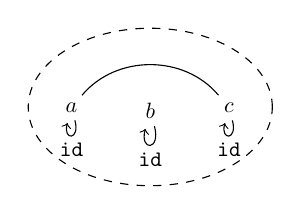
\begin{tikzpicture}[scale=0.5,every node/.style={scale=0.8}]
  \draw[dashed] (0,-0.3) ellipse (3.1cm and 2cm);
  \node[below] (A) at (-2,0) {$a$};
  \node[below] (B) at (0,0) {$b$};
  \node[below] (C) at (2,0) {$c$};
  \path (A) edge [bend left=50] (C); 
  \path (A) edge [loop below] node[below] {\texttt{id}} (A);
  \path (B) edge [loop below] node[below] {\texttt{id}} (B);
  \path (C) edge [loop below] node[below] {\texttt{id}} (C);
\end{tikzpicture}
\qquad 
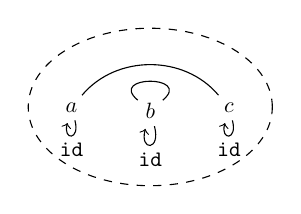
\begin{tikzpicture}[scale=0.5,every node/.style={scale=0.8}]
  \draw[dashed] (0,-0.3) ellipse (3.1cm and 2cm);
  \node[below] (A) at (-2,0) {$a$};
  \node[below] (B) at (0,0) {$b$};
  \node[below] (C) at (2,0) {$c$};
  \path (A) edge [bend left=50] (C); 
  \path (B) edge [out=140, in=40, looseness=4] (B);
  \path (A) edge [loop below] node[below] {\texttt{id}} (A);
  \path (B) edge [loop below] node[below] {\texttt{id}} (B);
  \path (C) edge [loop below] node[below] {\texttt{id}} (C);
\end{tikzpicture}
\end{center}





We want our computations to be information-preserving. Since the
amount of information in each state is just the log of the cardinality
of the space, computation just needs to be between spaces of the same
cardinality. 

\amr{from popl 12 paper: adapt}

Now consider the \ensuremath{\mathit{bool} \rightarrow \mathit{bool}}
function \ensuremath{\mathit{not}}. Let $p_F$ and $p_T$ be the
probabilities that the input is \ensuremath{\mathit{false}} or
\ensuremath{\mathit{true}} respectively. The outputs occur with the
reverse probabilities, i.e., $p_T$ is the probability that the output
is \ensuremath{\mathit{false}} and $p_F$ is the probability that t he
output is \ensuremath{\mathit{true}}. Hence the output entropy of the
function is $- p_F \log{p_F} - p_T \log{p_T}$ which is the same as the
input entropy and the function is information-preserving. As another
example, consider the \ensuremath{\mathit{bool} \rightarrow
  \mathit{bool}} function \ensuremath{\mathit{constT}(x) =
  \mathit{true}} which discards its input.  The output of the function
is always \ensuremath{\mathit{true}} with no uncertainty, which means
tha t the output entropy is 0, and that the function is not
information-preserving. As a third example, consider the
function~\ensuremath{\mathit{and}} and let the inputs occur with equal
probabilities, i.e., let the entropy of the input be 2. The output is
\ensuremath{\mathit{false}} with probability $3/4$ and
\ensuremath{\mathit{true}} with probability $1/4$, which means that
the output entropy is about 0.8 and the function is not
information-preserving. As a final example, consider the
\ensuremath{\mathit{bool} \rightarrow \mathit{bool}\times
  \mathit{bool}} function \ensuremath{\mathit{fanout} ~(x) = (x,x)}
which duplicates its input.  Let the input be
\ensuremath{\mathit{false}} with probability $p_F$ and
\ensuremath{\mathit{true}} be probability $p_T$. The output is
\ensuremath{(\mathit{false},\mathit{false})} with probability $p_F$
and \ensuremath{(\mathit{true},\mathit{true})} with probability $p_T$
which means that the output entropy is the same as the input entropy
and the function is information-preserving.

We are now ready to formalize the connection between reversibility and
entropy, once we define logical reversibility of computations. 

\begin{definition}[Logical reversibility~\cite{Zuliani:2001:LR}]
A function $f : b_1 \rightarrow b_2$ is logically reversible if there exists
an inverse function $g : b_2 \rightarrow b_1$ such that for all values $v_1
\in b_1$ and $v_2 \in b_2$, we have: $f(v_1) = v_2$ iff $g(v_2) = v_1$.
\end{definition}

\noindent The main proposition that motivates and justifies our approach is that
logically reversible functions are information-preserving.

\begin{proposition}
A function is logically reversible iff it is information-preserving.
\end{proposition}

Looking at the examples above, we argued that \ensuremath{\mathit{constT}}, \ensuremath{\mathit{and}} are
not information-preserving and that \ensuremath{\mathit{not}}, \ensuremath{\mathit{fanout}} are
information-preserving. As expected, neither \ensuremath{\mathit{constT}} nor \ensuremath{\mathit{and}}
are logically reversible and \ensuremath{\mathit{not}} is logically reversible. The
situation with \ensuremath{\mathit{fanout}} is however subtle and deserves some
explanation. First, note that the definition of logical reversibility
does not require the functions to be total, and hence it is possible
to define a \emph{partial} function \ensuremath{\mathit{fanin}} that is the logical
inverse of \ensuremath{\mathit{fanout}}. The function \ensuremath{\mathit{fanin}} maps \ensuremath{(\mathit{false},\mathit{false})}
to \ensuremath{\mathit{false}}, \ensuremath{(\mathit{true},\mathit{true})} to \ensuremath{\mathit{true}} and is undefined
otherwise. Arguing that partial functions like \ensuremath{\mathit{fanin}} are
information-preserving requires some care. Let the inputs to \ensuremath{\mathit{fanin}}
occur with equal probabilities, i.e., let the entropy of the input
be~2. Disregarding the partiality of \ensuremath{\mathit{fanin}}, one might reason that
the output is \ensuremath{\mathit{false}} with probability $1/4$ and \ensuremath{\mathit{true}} with
probability $1/4$ and hence that the output entropy is~1 which
contradicts the fact that \ensuremath{\mathit{fanin}} is logically reversible. The
subtlety is that entropy is defined with respect to observing some
probabilistic event: an infinite loop is not an event that can be
observed and hence the entropy analysis, just like the definition of
logical reversibility, only applies to the pairs of inputs and outputs
on which the function is defined. In the case of \ensuremath{\mathit{fanin}} this means
that the only inputs that can be considered are \ensuremath{(\mathit{false},\mathit{false})} and
\ensuremath{(\mathit{true},\mathit{true})} and in this case it is clear that the function is
information-preserving as expected.

\amr{end of popl 12 quote} 

%%%%%
\subsection{Constraints}

If we have the type $\mathsf{Bool} \times \mathsf{Bool}$ the
information in each state is 2 bits. But if our system also has a
constraint that the state must be of the form $(b,b)$, then there are
only possible states in the system and the information contained in
each is just one bit. There is a neat way to express the constraint
using an equivalence generated by a pi-program.
  
%%%%%
\subsection{Information Equivalence}
  
We need to show coherence of the definition of cardinalities on the
universe syntax with the Euler characteristic of the category which in
our case also corresponds to the groupoid cardinality. There are
several formulations and explanations. The following is quite simple
to implement: first collapse all the isomorphic objects. Then fix a
particular order of the objects and write a matrix whose $ij$'s entry
is the number of morphisms from $i$ to $j$. Invert the matrix. The
cardinality is the sum of the elements in the matrix.

Our notion of information equivalence is coarser than the conventional
notion of equivalence of categories (groupoids). This is fine as there
are several competing notions of equivalence of groupoids that are
coarser than strict categorical equivalence.

There are however other notions of equivalence of groupoids like
Morita equivalence and weak equivalence that we explore later. The
intuition of these weaker notions of equivalence is that two groupoids
can be considered equivalent if it is not possible to distinguish them
using certain observations. This informally corresponds to the notion
of ``observational equivalence'' in programming language
semantics. Note that negative entropy can only make sense locally in
an open system but that in a closed system, i.e., in a complete
computation, entropy cannot be negative. Thus we restrict
observational contexts to those in which fractional types do not
occur. Note that two categories can have the same cardinality but not
be equivalent or even Morita equivalent but the converse is
guaranteed. So it is necessary to have a separate notion of
equivalence and check that whenever we have the same cardinality, the
particular categories in question are equivalent.


